\documentclass{beamer}
%
% Choose how your presentation looks.
%
% For more themes, color themes and font themes, see:
% http://deic.uab.es/~iblanes/beamer_gallery/index_by_theme.html
%
\mode<presentation>
{
  \usetheme{Boadilla}      % or try Darmstadt, Madrid, Warsaw, ...
  \usecolortheme{beaver} % or try albatross, beaver, crane, ...
  \usefonttheme{default}  % or try serif, structurebold, ...
  \setbeamertemplate{navigation symbols}{}
  \setbeamertemplate{caption}[numbered]
  
} 

\usepackage{xcolor,colortbl}
\usepackage[english]{babel}
\usepackage[utf8x]{inputenc}
\usepackage{courier}
\usepackage{dsfont}
\usepackage{verbatim} 
\usepackage{enumerate}
\usepackage{tikz}
\usetikzlibrary{shapes.geometric, arrows}
\usepackage{multirow}
\usepackage{venndiagram}
\usepackage{epigraph} 
%\usepackage{xcolor}
\usepackage{makecell}

%\usepackage{enumitem}

\usepackage{hyperref}
\hypersetup{
    colorlinks=true,
    linkcolor=blue,
    filecolor=magenta,      
    urlcolor=cyan,
}

% R stuff!
\usepackage{listings}
\definecolor{codegreen}{rgb}{0,0.6,0}
\definecolor{codegray}{rgb}{0.5,0.5,0.5}
\definecolor{codepurple}{rgb}{0.58,0,0.82}
\definecolor{backcolour}{rgb}{0.95,0.95,0.92}

\lstdefinestyle{mystyle}{
    backgroundcolor=\color{backcolour},    
    commentstyle=\color{codegreen},
    keywordstyle=\color{black},
    numberstyle=\tiny\color{codegray},
    stringstyle=\color{codepurple},
    basicstyle=\ttfamily\footnotesize,
    breakatwhitespace=false,         
    breaklines=true,                 
    captionpos=b,                    
    keepspaces=true,                 
    numbers=left,                    
    numbersep=5pt,                  
    showspaces=false,                
    showstringspaces=false,
    showtabs=false,                  
    tabsize=2
}

\lstset{style=mystyle}


\setbeamertemplate{enumerate items}[default]
\setbeamertemplate{itemize item}[triangle]

%\setitemize{label=\usebeamerfont*{itemize item}%
%  \usebeamercolor[fg]{itemize item}
%  \usebeamertemplate{itemize item}}
\tikzstyle{startstop} = [rectangle, rounded corners, 
minimum width=3cm, 
minimum height=1cm,
text centered, 
draw=black, 
fill=red!30]

\tikzstyle{io} = [trapezium, 
trapezium stretches=true, % A later addition
trapezium left angle=70, 
trapezium right angle=110, 
minimum width=3cm, 
minimum height=1cm, text centered, 
draw=black, fill=blue!30]

\tikzstyle{process} = [rectangle, 
minimum width=3cm, 
minimum height=1cm, 
text centered, 
text width=3cm, 
draw=black, 
fill=orange!30]

\tikzstyle{decision} = [diamond, 
minimum width=3cm, 
minimum height=1cm, 
text centered, 
draw=black, 
fill=green!30]
\tikzstyle{arrow} = [thick,->,>=stealth]


\title[Introduction to Statistics]{Hypothesis Testing}
\subtitle{What other types of Questions can Statistics answer?}
\author{Grinnell College}
\date{}

\graphicspath{{img/}}

\begin{document}

\begin{frame}
  \titlepage
\end{frame}

\begin{frame}{Review -- Intervals}
We have been covering Confidence Intervals for a bit now. \vspace{8mm}

What was the purpose of confidence intervals?
\begin{itemize}
    \item estimating a parameter
\end{itemize} \vspace{8mm}

\textbf{Methods}
\begin{itemize}
    \item Normal methods ($p$, $p_1 - p_2$)
    \item t-distribution ($\mu$, $\mu_1-\mu_2$)
    \item bootstrap distribution (everything else)
\end{itemize}
\end{frame}

\begin{frame}{Answering Questions with CIs}
Sometimes when we had a confidence interval we would check whether a certain value was within that interval. \vspace{12mm}

\textbf{Example:} We want to find out if a coin is fair. We flip a coin a whole bunch and from our data we construct some confidence intervals. \vspace{4mm}

\textbf{90\% CI $\rightarrow$ (.47, .49)}
\begin{itemize}
    \item According to the CI, is the coin fair?
\end{itemize} \vspace{6mm}

\textbf{95\% CI $\rightarrow$ (.45, .51)}
\begin{itemize}
    \item According to the CI, is the coin fair?
\end{itemize}
\end{frame}

\begin{frame}{Answering Questions with CIs}
Sometimes when we had a confidence interval we would check whether a certain value was within that interval. \vspace{12mm}

Are there issues with this method? Yes!
\begin{itemize}
    \item Our answer depends on the confidence level of our CI
\end{itemize}
\end{frame}

\begin{frame}{Court Case}
Suppose you are selected to be on a jury to determine if someone is a murderer.

\hrulefill

What assumption do we make before the trial? \vspace{5mm}

What are the two decisions we can make? \vspace{5mm}

What do we use to make that decision? \vspace{5mm}

How much evidence do we need to make a conviction? \vspace{5mm}

If we find someone "not guilty" does that really mean they are "not guilty?" \vspace{5mm}

If we find someone "guilty" does that really mean they are "guilty?"
\vspace{5mm}
\end{frame} 

\begin{frame}{Hypothesis Testing}
\textbf{Hypothesis Testing} is the term we are going to give for figuring out how to answer binary questions using data \vspace{8mm}

\textbf{Examples}
\begin{itemize}
    \item is someone a murderer? (guilty / not guilty)
    \item is a coin fair? (yes / no)
    \item is a new drug better than existing drugs? (yes / no)
\end{itemize} \vspace{6mm}

\textbf{Note:} this process does not work for prediction
\begin{itemize}
    \item ex) will it rain tomorrow?
\end{itemize}
\end{frame}

\begin{frame}{Types of Questions in Statistics}
So far we have broadly encountered two scenarios in stats.
\begin{itemize}
    \item we want to estimate something (a parameter)
    \item we want to answer a binary question about a population
\end{itemize} \vspace{10mm}

For the remainder of the semester, I want you think about Research Questions that we formulate with this idea in mind...
\end{frame}

\begin{frame}{Which method to use?}
\begin{center}
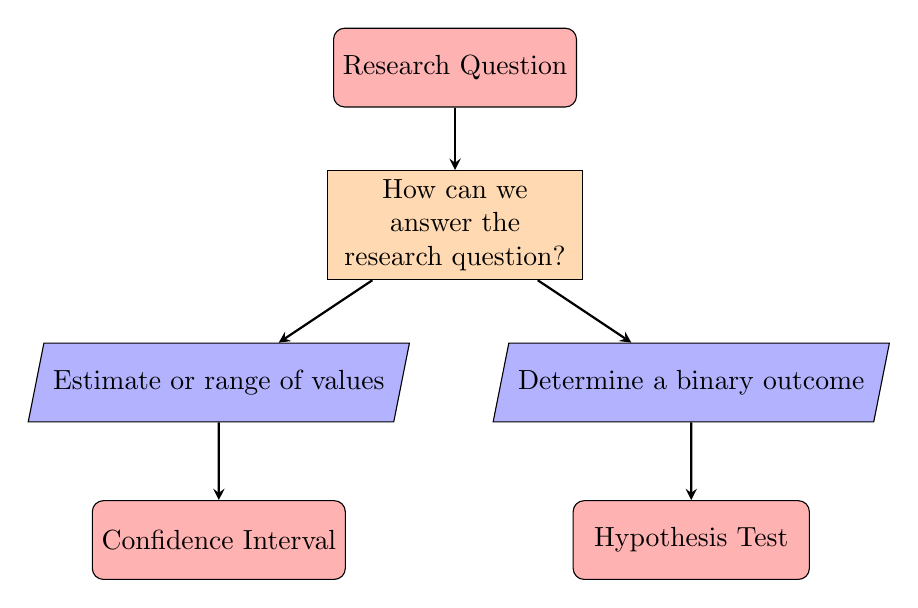
\begin{tikzpicture}[node distance=2cm]

\node (RQ) [startstop] {Research Question};
\node (pro1) [process, below of=RQ] {How can we answer the research question?};
\node (io1) [io, below of=pro1, xshift=-3cm] {Estimate or range of values};
\node (io2) [io, below of=pro1, xshift=3cm] {Determine a binary outcome};
\node (stop1) [startstop, below of=io1] {Confidence Interval};
\node (stop2) [startstop, below of=io2] {Hypothesis Test};
\draw [arrow] (RQ) -- (pro1);
\draw [arrow] (pro1) -- (io1);
\draw [arrow] (pro1) -- (io2);
\draw [arrow] (io1) -- (stop1);
\draw [arrow] (io2) -- (stop2);

\end{tikzpicture}
\end{center}
\end{frame}

\begin{frame}{Parameters and Statistics}
\textbf{Parameters} are numerical summaries of the population

\textbf{Statistics} are numerical summaries of the sample
\vspace{8mm}

Typically we will use special notation to differentiate \textit{population parameters} (things we wish to know) from \textit{statistics} computed from our sample:

\begin{table}[ht]
\centering
\begin{tabular}{rcc}
  \hline
 & Population Parameter & Sample Statistic \\ 
  \hline
Mean &   $\mu$ &   $\overline{x}$ \\ 
Standard Deviation &  $\sigma$ &   $s$ \\ 
Proportion & $p$ & $\hat{p}$ \\
Correlation & $\rho$ & $r$ \\
Regression & $\beta$ & $b$'s or $\hat{\beta}$'s \\
   \hline
\end{tabular}
\end{table} \vspace{2mm}
\begin{itemize}
    \item It is EXTREMELY important that you can define the parameter and statistic in context from here on out
    \item failure to do so means we can't even start hypothesis testing
\end{itemize}
\end{frame}

\begin{frame}{Parameters and Statistics}
For the rest of hypothesis testing (until told otherwise), we are going to focus on these four specific scenarios and the following parameters
\begin{itemize}
    \item population mean ($\mu$)
    \item difference in population means ($\mu_1 - \mu_2$)
    \item population proportion (p)
    \item difference in population means ($p_1 - p_2$)
\end{itemize}
\end{frame}

\begin{frame}{Which parameters to use?}
\begin{center}
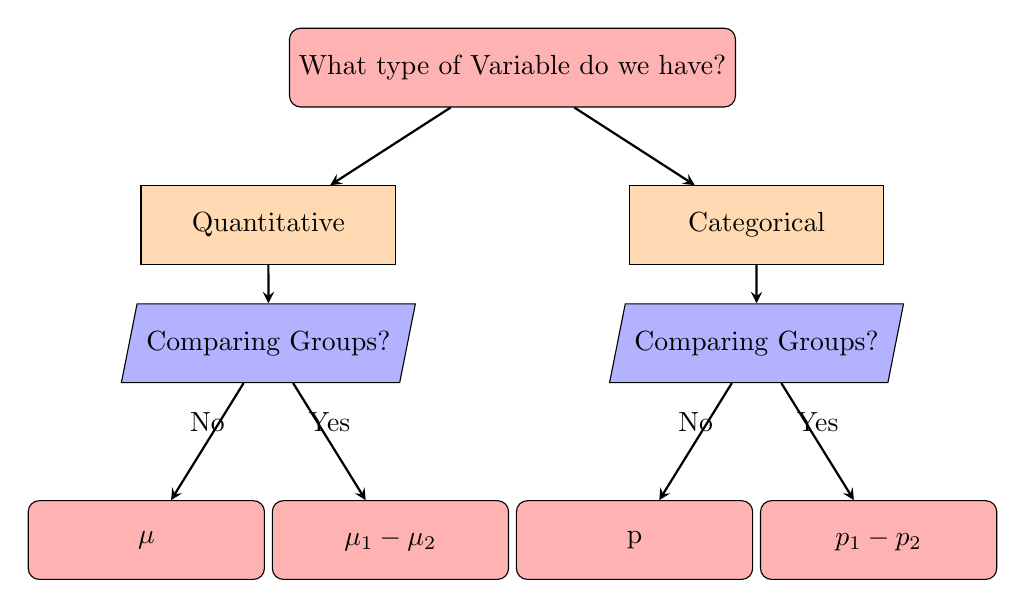
\begin{tikzpicture}[node distance=2cm]

\node (Var) [startstop] {What type of Variable do we have?};

\node (quant) [process, below of=Var, xshift=-3.1cm] {Quantitative};
\node (group1) [io, below of=quant, yshift=.5cm] {Comparing Groups?};

\node (cat) [process, below of=Var, xshift=3.1cm] {Categorical};
\node (group2) [io, below of=cat, yshift=.5cm] {Comparing Groups?};

\node (stop1) [startstop, below of=group1, xshift=-1.55cm, yshift=-.5cm] {$\mu$};
\node (stop2) [startstop, below of=group1, xshift=1.55cm, yshift=-.5cm] {$\mu_1 - \mu_2$};

\node (stop3) [startstop, below of=group2, xshift=-1.55cm, yshift=-.5cm] {p};
\node (stop4) [startstop, below of=group2, xshift=1.55cm, yshift=-.5cm] {$p_1 - p_2$};

\draw [arrow] (Var) -- (quant);
\draw [arrow] (Var) -- (cat);
\draw [arrow] (quant) -- (group1);
\draw [arrow] (cat) -- (group2);
\draw [arrow] (group1) -- node[anchor=south] {No} (stop1);
\draw [arrow] (group1) -- node[anchor=south] {Yes} (stop2);
\draw [arrow] (group2) -- node[anchor=south] {No} (stop3);
\draw [arrow] (group2) -- node[anchor=south] {Yes} (stop4);

\end{tikzpicture}
\end{center}
\end{frame}

\begin{frame}{Hypothesis Statements}
There are two possible outcomes for testing a research question.
\begin{itemize}
    \item The data supports the research question
    \item The data \textit{does not} support the research question
\end{itemize} \vspace{12mm}

A \textbf{Hypothesis Statement} is a statement about a parameter based on the research question.
\end{frame}

\begin{frame}{The Null Hypothesis}
\textbf{Null Hypothesis} -- hypothesis statement that represents an assumption of \underline{no effect} or \underline{no relationship} or \underline{no difference} between variables (status-quo)
\begin{itemize}
    \item uses the most basic assumption we can make about a parameter
    \item sometimes based on previous information
    \item denoted H$_0$ (H-"naught" or H-"oh" or H-zero)
\end{itemize} \vspace{8mm}

Form will always be...
\begin{itemize}
    \item H$_0$: parameter = 'hypothesized value'
    \item "our null hypothesis is that the parameter equals the hypothesized value"
    \item 'hypothesized value' is often written as the parameter with a 0 subscript
    \begin{itemize}
        \item ex) $\mu_0$, p$_0$
    \end{itemize}
\end{itemize}
\end{frame}

\begin{frame}{Null Hypothesis Examples}
Common examples include: \vspace{3mm}
\begin{itemize}
\item Testing if a pop. mean is equal to zero:
\begin{align*}
H_0: \mu = \mu_0 = 0
\end{align*}
\item Testing if difference of proportions between groups is zero
\begin{align*}
H_0: p_A - p_B = p_0 = 0
\end{align*}
\item Testing if odds ratio is equal to one (won't spend time on this):
\begin{align*}
H_0: \theta = \theta_0 = 1
\end{align*}
\end{itemize}
\end{frame}

\begin{frame}{The Alternative Hypothesis}
\textbf{Alternate Hypothesis} -- a hypothesis statement that represents what we want to show with evidence, based on the research question
\begin{itemize}
    \item claim we want to find evidence for
    \item denoted H$_A$
\end{itemize} \vspace{8mm}

Will look similar to H$_0$ but with a change.
\begin{itemize}
    \item H$_A$: parameter $<$ 'hypothesized value' (left-tailed test) \textbf{\underline{OR}}
    \item H$_A$: parameter $>$ 'hypothesized value' (right-tailed test) \textbf{\underline{OR}}
    \item H$_A$: parameter $\neq$ 'hypothesized value' (two-tailed test)
\end{itemize} \vspace{6mm}

The research question will determine which of these we actually use
\begin{itemize}
    \item always same hypothesized value as H$_0$
\end{itemize}

\end{frame}

\begin{frame}{Coin Flip Example}
Let's go back to testing the fairness of a coin. What is the best possible guess we could give for the 'true proportion of heads' a coin will land on if we haven't yet tested a coin? 
\vspace{4mm}

Research Question: Is the coin biased in favor of heads?

\hrulefill
\vspace{2mm}

What type of parameter will we work with to test this? \vspace{12mm}

Define the Null hypothesis for this research question \vspace{12mm}

Define the Alternative hypothesis for this research question \vspace{12mm}
\end{frame}

\begin{frame}{Coin Flip Example}
Research Question: Is the coin biased in favor of heads? \vspace{12mm}

How would we go about testing this question? Let's say we flip the coin 10 times.
\begin{itemize}
    \item We expect to get a proportion of heads around 0.5 if the coin is fair (hypothesized value)
    \item Will we get exactly $\widehat{p} = .5$ every time even if the coin is fair?
    \item What '\# heads'/10 would make you think the coin is unfair?
\end{itemize}
\end{frame}

\begin{frame}{Coin Flip Simulation}
We are going to simulate a bunch of coin flips. \vspace{14mm}

Go to "https://flipsimu.com/"
\begin{itemize}
    \item at the bottom, adjust the \# of coin flips to 10
    \item flip the coins and compute the sample proportion of heads $\widehat{p}$
    \item do it again
    \item mark results on the board
\end{itemize}
    
\end{frame}

\begin{frame}{Coin Flip Example}
This resulting distribution is called a "Null Distribution".
\begin{itemize}
    \item it simulates what results would look like if H$_0$ is really true.
\end{itemize} \vspace{8mm}

What shape do we see? \vspace{8mm}

What is the center of the distribution close to?
\begin{itemize}
    \item What name did we give to this value?
\end{itemize}\vspace{8mm}
\end{frame}

\begin{frame}{Coin Flip Example}
This resulting distribution is called a "Null Distribution".
\begin{itemize}
    \item it simulates what results would look like if H$_0$ is really true.
\end{itemize} \vspace{8mm}

What shape do we see? \textbf{Normal} \vspace{8mm}

What is the center of the distribution close to? \textbf{0.5}
\begin{itemize}
    \item What name did we give to this value? \textbf{hypothesized value}
\end{itemize}\vspace{8mm}
\end{frame}

\begin{frame}{Coin Flip Example}
\textbf{Goal:} Finding out if $p > 0.5$ \vspace{4mm}

Let's say I flipped the coin in question 10 times and got 8 heads
\begin{itemize}
    \item this means $\widehat{p} = .8$
    \item where is 0.8 on our randomization distribution? Is this rare?
\end{itemize} \vspace{8mm}

What is the probability of getting this result or a result more extreme? ($\widehat{p} \geq 0.8$)
\begin{itemize}
    \item these are the values that provide just as much, if not more, evidence against the coin being fair
    \item this has a special name: \textbf{p-value} (short for 'probability-value')
\end{itemize} \vspace{8mm}
\end{frame}

\begin{frame}{Coin Flip Example}
If we have $\widehat{p}$ = 0.8, we get a p-value of: \vspace{6mm}

What if we had $\widehat{p}$ = 0.9?
\begin{itemize}
    \item p-value =
    \item is this stronger or weaker evidence that the coin is not fair?
\end{itemize}
\end{frame}

\begin{frame}{Coin Flip Example}
What if we had even more trials of the 10 coin flips?
\begin{center}
    \includegraphics[scale=.6]{img/coin_null_distr.jpg}
\end{center}
\end{frame}

\begin{frame}{Coin Flip Example}
With $\widehat{p} = .8$, what is the p-value?
\begin{center}
    \includegraphics[scale=.6]{img/pvalue2.jpg}
\end{center}
\end{frame}

\begin{frame}{Null Distribution}
When we calculate p-values we are always going to do so using a distribution that simulates what the null hypothesis would look like
\begin{itemize}
    \item compare our statistic to the null distribution
    \item compute p-value using the sign in the alternate hypothesis
\end{itemize} \vspace{8mm}

\textbf{Null Distribution}:

The distribution of the statistics if the null hypothesis is true
\begin{itemize}
    \item simulates what the null hypothesis looks like
\end{itemize} \vspace{8mm}
\end{frame}

\begin{frame}{P-values}
\textbf{P-values} are a way of quantifying how strong the evidence is \textit{against} the Null Hypothesis
\begin{itemize}
    \item equivalently: how strong the evidence is \textit{in support} of the Alternative Hypothesis
\end{itemize} \vspace{6mm}

\underline{Formal definition}:

The probability of getting an observed statistic equal to or more extreme than what we got \textit{IF THE NULL HYPOTHESIS IS TRUE}
\begin{itemize}
    \item this is a conditional probability
\end{itemize} \vspace{6mm}

\textbf{Interpretation:}
\begin{itemize}
    \item 'More extreme' = contrary to the Null hypothesis
    \item 'More extreme' is defined by the alternative hypothesis
    \item smaller p-value $\rightarrow$ more evidence against H$_0$
    \item smaller p-value $\rightarrow$ more evidence in favor of H$_A$
\end{itemize}
\end{frame}

\begin{frame}{How do we quantify the evidence strength?}
To do this we will look at the p-value. "Where does it fall on this chart?"
\begin{center}
    \includegraphics[scale=.6]{img/strength_chart.jpg}
\end{center}
$\widehat{p} = 0.8 \rightarrow$ p-value = 0.052
\end{frame}

\begin{frame}{Coin Flip Example}
With $\widehat{p} = .8$, the p-value of 0.052 indicates there is borderline or weak evidence against the Null hypothesis
\begin{itemize}
    \item Null hypothesis: coin is fair
    \item $\widehat{p} = .8$ is not particularly rare in a trial of 10 flips $\rightarrow$ weak evidence to say the coin is biased in favor of heads
\end{itemize} \vspace{12mm}

\textbf{Conclusion:} there is weak evidence that the coin is biased in favor of heads
\end{frame}

\begin{frame}{P-value Interpretation}
\textbf{Interpretation}:

(value of the p-value) is the probability of getting a (statistic) of (statistic value) or more if (null hypothesis) is true
\begin{itemize}
    \item replace placeholders with our values and context
    \item basically just saying the definition of a p-value with values and context
\end{itemize} \vspace{8mm}

\textbf{Conclusion}: 
\begin{itemize}
    \item mention strength of evidence, parameter, and context
    \item try to answer the research question with our evidence
\end{itemize}
There is (strength) evidence that the (parameter) is (pick $>$, $<$, $\neq$) the hypotheized value
\end{frame}


\begin{frame}{Central Limit Theorem}
When certain conditions are met (normal pop. or large sample size), we saw that the sampling distribution of means and proportions is a Normal distribution. \vspace{12mm}

We will use this as the starting point for constructing null distributions.
\end{frame}

\begin{frame}{Null Distribution -- Proportion}
Conditions:
\begin{itemize}
    \item Random Sample
    \begin{itemize}
        \item this doesn't affect our null distr. but makes sure answers are accurate
    \end{itemize}
    \item np$_0 >$ 10
    \item n(1 - p$_0) >$ 10
\end{itemize} \vspace{4mm}

With the conditions met, the null distribution for $\widehat{p}$ looks like this:
\begin{align*}
    \widehat{p} \sim N(p_0, \sqrt{\frac{p_0(1 - p_0)}{n}})
\end{align*}
\begin{itemize}
    \item use pnorm() to get p-values with these values for mean \& std. dev.
\end{itemize} \vspace{2mm}
\textbf{Note:} we have p$_0$'s in the distribution because we are simulating what the null hypothesis looks like
\end{frame}


\begin{frame}{Wrapping up}
What kinds of questions can we answer with CIs? \vspace{8mm}

What kinds of questions can we answer with hypothesis tests? \vspace{8mm}

What does a null distribution show us?
\vspace{8mm}

Broadly, what do p-values tell us?
\end{frame}
%%%%%%%%%%%%%%%%

%\begin{frame}
%\begin{columns}
%
%  \begin{column}{0.45\textwidth}
%%
%  \end{column}
%  \begin{column}{0.45\textwidth}
%%
%  \end{column}
%
%\end{columns}
%\end{frame}


\end{document}

\begin{frame}{Finding P-values}
When calculating a p-value you must ALWAYS look at the sign in the alternative hypothesis. This determines the direction in which you find the area. Then look at the null distribution and find where the statistic value is\vspace{4mm}

H$_A$: parameter $>$ 'hypothesized value'
\begin{itemize}
    \item Find area 'greater than' the statistic on the null distribution
    \item "right-tailed test"
\end{itemize} \vspace{4mm}

H$_A$: parameter $<$ 'hypothesized value'
\begin{itemize}
    \item Find area 'less than' the statistic on the null distribution
    \item "left-tailed test"
\end{itemize} \vspace{4mm}

H$_A$: parameter $\neq$ 'hypothesized value'
\begin{itemize}
    \item Find area 'greater than' the statistic (if statistic is positive) and area 'less than' -statistic
    \item "two-tailed test"
\end{itemize} \vspace{4mm}
\end{frame}

\begin{frame}{Coin P-value Example 1}
H$_A$: p $\neq 0.5$, with $\widehat{p} = .8$, the p-value is 0.057 + .057 = 0.114
\begin{center}
    \includegraphics[scale=.55]{img/coin_pvalue.jpg}
\end{center}
\end{frame}

\begin{frame}{Coin P-value Example 2}
H$_A$: p $> 0.5$, with $\widehat{p} = .8$, the p-value is 0.052
\begin{center}
    \includegraphics[scale=.55]{img/pvalue2.jpg}
\end{center}
\end{frame}

\begin{frame}{Coin P-value Example 3}
H$_A$: p $< 0.5$, with $\widehat{p} = .8$, the p-value is 0.99
\begin{center}
    \includegraphics[scale=.55]{img/pvalue1.jpg}
\end{center}
\end{frame}

\begin{frame}{Test-Statistic}
For null distributions, we will use the Normal and t-distribution stuff like we did with CI's, but with a small twist... \vspace{8mm}

To make things, easier, we are going to calculate something called a "test-statistic" that will help us in calculating p-values.
\begin{itemize}
    \item will always be labeled with a Z or a T
\end{itemize} \vspace{8mm}

The test-statistic is a value we calculate and are going to use with the pnorm() or pt() functions in R to get p-values \vspace{6mm}

It will always have the form: \vspace{2mm}

test-statistic = $\frac{\text{statistic - hypothesized value}}{\text{standard error}}$
\end{frame}

\begin{frame}{Hypothesis Test -- Single Proportion}
H$_0$: p = p$_0$ \vspace{4mm}

Under the null hypothesis we have:
\begin{equation*}
    Z := \frac{\widehat{p} - p_0}{\sqrt{\frac{p_0(1-p_0)}{n}}} \sim \textbf{N(0,1)}
\end{equation*} \vspace{-4mm}
\begin{itemize}
    \item use pnorm() with value of Z
\end{itemize} \vspace{4mm}

\textbf{Conditions:}
\begin{itemize}
    \item Random Sample
    \item $n \times p_0 \geq 10$
    \item $n \times (1-p_0) \geq 10$
\end{itemize}
\end{frame}